% =============================================================================
% relatorio_fsm.tex -- Relatorio: Maquina de Estado Finita (FSM)
% Unidade 5 | Capitulo 2 | Capacitacao Profissional em Microeletronica (PADIS)
% Autor : Matheus Serrao Uchoa   Matricula: 22052633
% Prof. : Alexandre Almeida
% =============================================================================
\documentclass[12pt,a4paper]{article}

% ---------------------------------------------------------------------------
% Pacotes
% ---------------------------------------------------------------------------
\usepackage[utf8]{inputenc}
\usepackage[T1]{fontenc}
\usepackage[brazil]{babel}
\usepackage{lmodern}
\usepackage{geometry}
\usepackage{graphicx}
\usepackage{booktabs}
\usepackage{array}
\usepackage{multirow}
\usepackage{amsmath}
\usepackage{amssymb}
\usepackage{xcolor}
\usepackage{hyperref}
\usepackage{fancyhdr}
\usepackage{titlesec}
\usepackage{caption}
\usepackage{subcaption}
\usepackage{float}
\usepackage{enumitem}
\usepackage[most]{tcolorbox}
\usepackage{listings}
\usepackage{tikz}
\usetikzlibrary{arrows.meta, positioning, shapes.geometric, automata, fit, calc}

\geometry{top=2.5cm, bottom=2.5cm, left=3cm, right=2.5cm}

% ---------------------------------------------------------------------------
% Cores
% ---------------------------------------------------------------------------
\definecolor{azulpadis}{RGB}{0,82,155}
\definecolor{verdepadis}{RGB}{0,130,79}
\definecolor{cinzaclaro}{RGB}{245,245,245}
\definecolor{cinzaborda}{RGB}{180,180,180}
\definecolor{codebg}{RGB}{252,252,252}
\definecolor{codeframe}{RGB}{180,180,200}
\definecolor{kw}{RGB}{0,0,180}
\definecolor{cm}{RGB}{60,120,60}
\definecolor{st}{RGB}{163,21,21}

% ---------------------------------------------------------------------------
% Estilo de pagina
% ---------------------------------------------------------------------------
\pagestyle{fancy}
\fancyhf{}
\fancyhead[L]{\small\textcolor{azulpadis}{\textbf{PADIS -- Microeletronica}}}
\fancyhead[R]{\small\textcolor{azulpadis}{Unidade 5 | Cap.\ 2 -- FSM}}
\fancyfoot[C]{\small\thepage}
\renewcommand{\headrulewidth}{0.4pt}

% ---------------------------------------------------------------------------
% Titulos
% ---------------------------------------------------------------------------
\titleformat{\section}{\large\bfseries\color{azulpadis}}{{\thesection.}}{0.5em}{}[\titlerule]
\titleformat{\subsection}{\normalsize\bfseries\color{azulpadis}}{{\thesubsection}}{0.5em}{}
\titleformat{\subsubsection}{\normalsize\bfseries\color{verdepadis}}{{\thesubsubsection}}{0.5em}{}

% ---------------------------------------------------------------------------
% tcolorbox: caixas de destaque
% ---------------------------------------------------------------------------
\tcbuselibrary{skins, breakable}

\newtcolorbox{destaquebox}[1][]{
  enhanced, breakable,
  colback=cinzaclaro, colframe=azulpadis,
  fonttitle=\bfseries\small, title=#1,
  boxrule=0.6pt, arc=3pt,
  left=4pt, right=4pt, top=4pt, bottom=4pt
}

\newtcolorbox{unidadebox}[1][]{
  enhanced, breakable,
  colback=blue!4!white, colframe=azulpadis!70,
  fonttitle=\bfseries\small\color{azulpadis},
  title=#1,
  boxrule=0.5pt, arc=3pt,
  left=5pt, right=5pt, top=4pt, bottom=4pt
}

% ---------------------------------------------------------------------------
% Listings -- SystemVerilog
% ---------------------------------------------------------------------------
\lstdefinelanguage{SystemVerilog}{
  morekeywords={module,endmodule,parameter,input,output,logic,always_comb,
    always_ff,typedef,enum,posedge,negedge,begin,end,case,endcase,
    unique,if,else,default,assign,wire,reg,int,initial,task,endtask,
    automatic,timescale},
  sensitive=true,
  morecomment=[l]{//},
  morecomment=[s]{/*}{*/},
  morestring=[b]"
}

\lstset{
  language=SystemVerilog,
  backgroundcolor=\color{codebg},
  frame=single,
  rulecolor=\color{codeframe},
  basicstyle=\ttfamily\footnotesize,
  keywordstyle=\color{kw}\bfseries,
  commentstyle=\color{cm}\itshape,
  stringstyle=\color{st},
  numbers=left,
  numberstyle=\tiny\color{gray},
  numbersep=6pt,
  tabsize=4,
  breaklines=true,
  showstringspaces=false,
  captionpos=b,
  xleftmargin=12pt,
  xrightmargin=4pt
}

% ---------------------------------------------------------------------------
% Hifenizacao
% ---------------------------------------------------------------------------
\hyphenation{Micro-ele-tro-ni-ca Se-quen-cia-dor}

% ===========================================================================
% DOCUMENTO
% ===========================================================================
\begin{document}

% ---------------------------------------------------------------------------
% CAPA
% ---------------------------------------------------------------------------
\begin{titlepage}
  \centering
  \vspace*{1cm}

  {\Large\bfseries\color{azulpadis}
    Programa de Apoio ao Desenvolvimento da Indústria de Semicondutores\\[4pt]
    \textsc{PADIS} -- Capacitação em Microeletrônica}

  \vspace{0.4cm}
  \textcolor{cinzaborda}{\rule{\linewidth}{1.2pt}}
  \vspace{0.8cm}

  {\LARGE\bfseries Unidade 5 | Capítulo 2\\[6pt]
   Máquina de Estado Finita (FSM)\\[4pt]
   Detector de Sequência Serial ``101''}

  \vspace{0.8cm}
  \textcolor{cinzaborda}{\rule{\linewidth}{0.6pt}}

  \vspace{1.2cm}
  \begin{center}
    \begin{tikzpicture}[node distance=1.8cm, >=Stealth,
        state/.style={circle, draw=azulpadis, thick, minimum size=1.2cm,
                      font=\small\bfseries, fill=blue!6}]
      \node[state, initial, initial text=reset] (S0) {IDLE};
      \node[state, right=of S0] (S1) {GOT1};
      \node[state, right=of S1] (S2) {GOT10};
      \node[state, accepting, right=of S2, fill=verdepadis!15, draw=verdepadis] (S3) {GOT101};

      \draw[->] (S0) edge[loop above] node[above,font=\tiny]{0} (S0);
      \draw[->] (S0) edge[bend left=20] node[above,font=\tiny]{1} (S1);
      \draw[->] (S1) edge[loop above] node[above,font=\tiny]{1} (S1);
      \draw[->] (S1) edge[bend left=20] node[above,font=\tiny]{0} (S2);
      \draw[->] (S2) edge[bend left=40] node[below,font=\tiny]{0} (S0);
      \draw[->] (S2) edge[bend left=20] node[above,font=\tiny]{1} (S3);
      \draw[->] (S3) edge[bend left=40] node[above,font=\tiny]{0} (S2);
      \draw[->] (S3) edge[bend right=45] node[below,font=\tiny]{1} (S1);
    \end{tikzpicture}
  \end{center}

  \vspace{0.8cm}
  \textcolor{cinzaborda}{\rule{\linewidth}{0.6pt}}
  \vspace{0.8cm}

  \begin{tabular}{rl}
    \textbf{Aluno:} & Matheus Serrão Uchôa -- Matrícula: 22052633 \\[4pt]
    \textbf{Professor:} & Alexandre Almeida \\[4pt]
    \textbf{Curso:} & Capacitação Profissional em Microeletrônica (PADIS) \\[4pt]
    \textbf{Instituição:} & Universidade Federal do Amazonas (UFAM) \\[4pt]
    \textbf{Data:} & Maio de 2026
  \end{tabular}
\end{titlepage}

% ---------------------------------------------------------------------------
\tableofcontents
\newpage

% ===========================================================================
\section{Introdução}
% ===========================================================================

As \textbf{Máquinas de Estado Finitas} (FSM -- \textit{Finite State Machine}) constituem
um dos pilares do projeto digital moderno. Presentes em controladores de protocolo,
decodificadores de fluxo serial e interfaces de memória, as FSMs permitem descrever
comportamentos sequenciais complexos de forma sistemática, diretamente sintetizável
em FPGA e ASIC.

Este relatório apresenta o projeto, simulação e análise de dois detectores de sequência
serial ``101'' implementados em SystemVerilog IEEE 1800-2012: um seguindo o modelo
\textbf{Moore} e outro o modelo \textbf{Mealy}. Ambos utilizam o estilo de três
processos (\textit{three-process FSM}) recomendado pelo curso, com detecção com
sobreposição (\textit{overlapping}) e reset assíncrono ativo em nível baixo.

\begin{unidadebox}[Conexao com o Curso -- Unidade 5 / Capitulo 2: FSM]
  Esta atividade integra os conteúdos de lógica sequencial, linguagem SystemVerilog
  e fluxo de projeto digital. O detector de sequência exemplifica aplicações práticas
  das FSMs em protocolos de comunicação serial e decodificação de dados em sistemas
  embarcados de monitoramento, como o \textit{Aqua Monitor}.
\end{unidadebox}

% ===========================================================================
\section{Objetivos}
% ===========================================================================

\begin{itemize}[leftmargin=1.5cm]
  \item Implementar uma FSM do tipo \textbf{Moore} para detecção da sequência ``101''
        com sobreposição em SystemVerilog;
  \item Implementar uma FSM do tipo \textbf{Mealy} para o mesmo problema, com
        um estado a menos em relação à Moore;
  \item Comparar as duas arquiteturas quanto ao número de estados, latência de saída
        e comportamento de sobreposição;
  \item Verificar ambas as implementações por simulação com \textit{testbenches}
        automatizados (PASS/FAIL) usando a sequência de entrada \texttt{"11010010111"};
  \item Gerar formas de onda e documentar os resultados em relatório técnico.
\end{itemize}

% ===========================================================================
\section{Materiais e Ferramentas}
% ===========================================================================

\begin{table}[H]
  \centering
  \caption{Ferramentas utilizadas}
  \label{tab:ferramentas}
  \begin{tabular}{lll}
    \toprule
    \textbf{Ferramenta} & \textbf{Versão} & \textbf{Finalidade} \\
    \midrule
    Icarus Verilog (iverilog) & 12.0 & Compilação SystemVerilog (\texttt{-g2012}) \\
    VVP runtime               & 12.0 & Execução da simulação / geração de VCD \\
    GTKWave                   & 3.3  & Visualização das formas de onda (.vcd) \\
    Python / Matplotlib       & 3.11 / 3.8 & Geração de figuras para o relatório \\
    \LaTeX\ (pdflatex)        & TeX Live 2023 & Composição do relatório \\
    \bottomrule
  \end{tabular}
\end{table}

\subsection{Arquivos do Projeto}

\begin{itemize}[leftmargin=1.5cm]
  \item \texttt{sequence\_detector\_moore.sv} -- Implementação Moore (4 estados)
  \item \texttt{sequence\_detector\_mealy.sv} -- Implementação Mealy (3 estados)
  \item \texttt{tb\_moore.sv} -- Testbench para a FSM Moore
  \item \texttt{tb\_mealy.sv} -- Testbench para a FSM Mealy
  \item \texttt{gerar\_waveforms.py} -- Gerador de figuras de formas de onda
\end{itemize}

% ===========================================================================
\section{Fundamentos Teóricos}
% ===========================================================================

\subsection{Máquinas de Estado Finitas (FSM)}

Uma FSM é um modelo matemático que descreve um sistema por meio de:
\begin{itemize}[leftmargin=1.5cm]
  \item Um conjunto finito de \textbf{estados} $Q = \{q_0, q_1, \ldots, q_n\}$;
  \item Um \textbf{estado inicial} $q_0$;
  \item Um conjunto de \textbf{entradas} $\Sigma$;
  \item Uma \textbf{função de transição} $\delta: Q \times \Sigma \rightarrow Q$;
  \item Uma \textbf{função de saída} (modelo-dependente).
\end{itemize}

Os dois modelos principais diferem na forma como a saída é gerada:

\begin{table}[H]
  \centering
  \caption{Comparação Moore vs.\ Mealy}
  \label{tab:moore_vs_mealy}
  \begin{tabular}{lll}
    \toprule
    \textbf{Característica} & \textbf{Moore} & \textbf{Mealy} \\
    \midrule
    Saída depende de        & Estado atual apenas & Estado atual + Entrada atual \\
    Número de estados       & Geralmente maior    & Geralmente menor \\
    Latência da saída       & Após a borda de clock & Combinacional (mesmo ciclo) \\
    Sensibilidade a glitches & Baixa (síncrona) & Maior (saída combinacional) \\
    Diagrama de estados     & Saída marcada no estado & Saída marcada na transição \\
    \bottomrule
  \end{tabular}
\end{table}

\subsection{Detecção da Sequência ``101'' com Sobreposição}

Dado um fluxo serial de bits, o detector deve emitir \texttt{sequence\_detected = 1}
sempre que os três bits mais recentes formarem a padrão ``101''. O modo
\textbf{com sobreposição} (\textit{overlapping}) significa que o último ``1'' da
detecção anterior pode ser reaproveitado como início da próxima -- permitindo detectar,
por exemplo, ``\underline{101}0\underline{1}'' com detecção nos bits 1--3 e 3--5.

\subsection{Diagrama de Estados -- Moore FSM (4 estados)}

A figura~\ref{fig:moore_states} apresenta o diagrama de estados da FSM Moore.
A saída \texttt{sequence\_detected = 1} está associada ao estado \texttt{GOT101}.

\begin{figure}[H]
  \centering
  \begin{tikzpicture}[node distance=2.5cm, >=Stealth, auto,
      every state/.style={circle, draw=azulpadis, thick, minimum size=1.4cm,
                          font=\small\bfseries},
      accepting/.style={double, double distance=2pt}]

    \node[state, initial, initial text=rst\_n] (S0) {IDLE\\{\tiny out=0}};
    \node[state, right=of S0] (S1) {GOT1\\{\tiny out=0}};
    \node[state, right=of S1] (S2) {GOT10\\{\tiny out=0}};
    \node[state, accepting, right=of S2,
          fill=verdepadis!15, draw=verdepadis] (S3) {GOT101\\{\tiny out=1}};

    \draw[->] (S0) edge[loop above] node{0} (S0);
    \draw[->] (S0) edge[bend left=25] node{1} (S1);
    \draw[->] (S1) edge[loop above] node{1} (S1);
    \draw[->] (S1) edge[bend left=25] node{0} (S2);
    \draw[->] (S2) edge[bend left=35] node[below]{0} (S0);
    \draw[->] (S2) edge[bend left=25] node{1} (S3);
    \draw[->] (S3) edge[bend left=35] node[above]{0} (S2);
    \draw[->] (S3) edge[bend right=50] node[below]{1} (S1);
  \end{tikzpicture}
  \caption{Diagrama de estados da FSM Moore -- Detector de ``101''}
  \label{fig:moore_states}
\end{figure}

\subsection{Diagrama de Estados -- Mealy FSM (3 estados)}

Na FSM Mealy (figura~\ref{fig:mealy_states}), as saídas são indicadas nas
transições no formato \textit{entrada/saída}. O estado \texttt{GOT101} é eliminado:
a detecção ocorre diretamente na transição \texttt{GOT10} $\xrightarrow{1/1}$
\texttt{GOT1}, reduzindo o número de estados de 4 para 3.

\begin{figure}[H]
  \centering
  \begin{tikzpicture}[node distance=3cm, >=Stealth, auto,
      every state/.style={circle, draw=azulpadis, thick, minimum size=1.4cm,
                          font=\small\bfseries}]

    \node[state, initial, initial text=rst\_n] (S0) {IDLE};
    \node[state, right=of S0] (S1) {GOT1};
    \node[state, right=of S1] (S2) {GOT10};

    \draw[->] (S0) edge[loop above] node{0/0} (S0);
    \draw[->] (S0) edge[bend left=25] node{1/0} (S1);
    \draw[->] (S1) edge[loop above] node{1/0} (S1);
    \draw[->] (S1) edge[bend left=25] node{0/0} (S2);
    \draw[->] (S2) edge[bend left=30] node[below]{0/0} (S0);
    \draw[->] (S2) edge[bend right=50,
                        draw=verdepadis, thick] node[above, text=verdepadis]{1/\textbf{1}} (S1);
  \end{tikzpicture}
  \caption{Diagrama de estados da FSM Mealy -- Detector de ``101'' (formato: entrada/saída)}
  \label{fig:mealy_states}
\end{figure}

\subsection{Tabelas de Transição de Estado}

\subsubsection{Moore FSM}

\begin{table}[H]
  \centering
  \caption{Tabela de transição -- Moore FSM}
  \label{tab:trans_moore}
  \begin{tabular}{ccccc}
    \toprule
    \textbf{Estado Atual} & \textbf{Codif.} & \textbf{Entrada x=0} & \textbf{Entrada x=1} & \textbf{Saída} \\
    \midrule
    IDLE   & 2'b00 & IDLE   & GOT1   & 0 \\
    GOT1   & 2'b01 & GOT10  & GOT1   & 0 \\
    GOT10  & 2'b10 & IDLE   & GOT101 & 0 \\
    GOT101 & 2'b11 & GOT10  & GOT1   & \textbf{1} \\
    \bottomrule
  \end{tabular}
\end{table}

\subsubsection{Mealy FSM}

\begin{table}[H]
  \centering
  \caption{Tabela de transição -- Mealy FSM (formato: próximo estado / saída)}
  \label{tab:trans_mealy}
  \begin{tabular}{cccc}
    \toprule
    \textbf{Estado Atual} & \textbf{Codif.} & \textbf{x=0} & \textbf{x=1} \\
    \midrule
    IDLE  & 2'b00 & IDLE  / 0  & GOT1  / 0 \\
    GOT1  & 2'b01 & GOT10 / 0  & GOT1  / 0 \\
    GOT10 & 2'b10 & IDLE  / 0  & GOT1  / \textbf{1} \\
    \bottomrule
  \end{tabular}
\end{table}

\subsection{Estilo Três Processos em SystemVerilog}

O estilo de três processos (\textit{three-process FSM}) separa claramente:

\begin{enumerate}[leftmargin=1.5cm]
  \item \textbf{Processo 1 -- Registrador de Estado:} bloco \texttt{always\_ff}
        sensível à borda de subida do clock e à borda de descida do reset
        assíncrono (\texttt{rst\_n}). Garante que a transição de estado só ocorre
        na borda do clock ou mediante reset imediato.
  \item \textbf{Processo 2 -- Lógica de Próximo Estado:} bloco \texttt{always\_comb}
        com \texttt{unique case}. Descreve puramente a função de transição $\delta$,
        sem memória.
  \item \textbf{Processo 3 -- Lógica de Saída:} bloco \texttt{always\_comb} que
        implementa a função de saída. Na Moore, depende apenas do estado; na Mealy,
        depende do estado e da entrada.
\end{enumerate}

% ===========================================================================
\section{Implementação em SystemVerilog}
% ===========================================================================

\subsection{Moore FSM -- \texttt{sequence\_detector\_moore.sv}}

\lstinputlisting[
  caption={sequence\_detector\_moore.sv -- FSM Moore (4 estados)},
  label={lst:moore}
]{sequence_detector_moore.sv}

\subsection{Mealy FSM -- \texttt{sequence\_detector\_mealy.sv}}

\lstinputlisting[
  caption={sequence\_detector\_mealy.sv -- FSM Mealy (3 estados)},
  label={lst:mealy}
]{sequence_detector_mealy.sv}

% ===========================================================================
\section{Testbenches}
% ===========================================================================

\subsection{Sequência de Verificação}

A sequência de teste adotada é \texttt{"11010010111"}, composta por 11 bits.
A tabela~\ref{tab:seq_test} mostra a evolução de estados e a saída esperada
para cada modelo.

\begin{table}[H]
  \centering
  \caption{Evolução da sequência de teste \texttt{"11010010111"}}
  \label{tab:seq_test}
  \resizebox{\textwidth}{!}{%
  \begin{tabular}{ccccccc}
    \toprule
    \textbf{Ciclo} & \textbf{Bit (x)} & \textbf{Estado Moore} & \textbf{Saída Moore}
                   & \textbf{Estado Mealy} & \textbf{Saída Mealy} & \textbf{Evento} \\
    \midrule
    1  & 1 & GOT1   & 0 & GOT1  & 0 & -- \\
    2  & 1 & GOT1   & 0 & GOT1  & 0 & -- \\
    3  & 0 & GOT10  & 0 & GOT10 & 0 & -- \\
    4  & 1 & GOT101 & \textbf{1} & GOT1  & \textbf{1} & \textbf{Detecção \#1} \\
    5  & 0 & GOT10  & 0 & GOT10 & 0 & Sobreposição \\
    6  & 0 & IDLE   & 0 & IDLE  & 0 & -- \\
    7  & 1 & GOT1   & 0 & GOT1  & 0 & -- \\
    8  & 0 & GOT10  & 0 & GOT10 & 0 & -- \\
    9  & 1 & GOT101 & \textbf{1} & GOT1  & \textbf{1} & \textbf{Detecção \#2} \\
    10 & 1 & GOT1   & 0 & GOT1  & 0 & -- \\
    11 & 1 & GOT1   & 0 & GOT1  & 0 & -- \\
    \bottomrule
  \end{tabular}}
\end{table}

\noindent\textbf{Nota sobre o timing de saída:}
Na FSM Moore, a saída \texttt{sequence\_detected = 1} ocorre no ciclo 4 e 9,
\emph{após} a borda de subida que leva a FSM ao estado \texttt{GOT101}. Na FSM
Mealy, a saída é combinacional: vale 1 \emph{durante} o ciclo (quando estado =
\texttt{GOT10} e $x = 1$), antes da borda que registra a próxima transição.
Esta diferença de um ciclo de latência é uma característica fundamental que
diferencia os dois modelos.

\subsection{Testbench Moore -- \texttt{tb\_moore.sv}}

\lstinputlisting[
  caption={tb\_moore.sv -- Testbench para a FSM Moore},
  label={lst:tb_moore}
]{tb_moore.sv}

\subsection{Testbench Mealy -- \texttt{tb\_mealy.sv}}

\lstinputlisting[
  caption={tb\_mealy.sv -- Testbench para a FSM Mealy},
  label={lst:tb_mealy}
]{tb_mealy.sv}

% ===========================================================================
\section{Resultados de Simulação}
% ===========================================================================

\subsection{Compilação e Execução}

Os comandos utilizados para compilar e simular são:

\begin{lstlisting}[language=bash, caption={Compilação e simulação com Icarus Verilog},
                   label={lst:sim_cmd}]
# Moore
iverilog -g2012 -o sim_moore sequence_detector_moore.sv tb_moore.sv
vvp sim_moore

# Mealy
iverilog -g2012 -o sim_mealy sequence_detector_mealy.sv tb_mealy.sv
vvp sim_mealy
\end{lstlisting}

\subsection{Saída do Console -- Moore FSM}

\begin{lstlisting}[language={},
  caption={Log de simulação -- Moore FSM (11/11 ciclos corretos)},
  label={lst:log_moore},
  numbers=none, frame=single, backgroundcolor=\color{cinzaclaro}]
=== Simulacao Moore FSM -- Detector de Sequencia '101' ===
Sequencia de entrada: 1 1 0 1 0 0 1 0 1 1 1
Ciclo       x       detected      Esperado      Status
------------------------------------------------------------------------
  [OK]    Ciclo 1  | x=1 | detected=0 | Esperado=0
  [OK]    Ciclo 2  | x=1 | detected=0 | Esperado=0
  [OK]    Ciclo 3  | x=0 | detected=0 | Esperado=0
  [OK]    Ciclo 4  | x=1 | detected=1 | Esperado=1   <- DETECCAO #1
  [OK]    Ciclo 5  | x=0 | detected=0 | Esperado=0   (sobreposicao)
  [OK]    Ciclo 6  | x=0 | detected=0 | Esperado=0
  [OK]    Ciclo 7  | x=1 | detected=0 | Esperado=0
  [OK]    Ciclo 8  | x=0 | detected=0 | Esperado=0
  [OK]    Ciclo 9  | x=1 | detected=1 | Esperado=1   <- DETECCAO #2
  [OK]    Ciclo 10 | x=1 | detected=0 | Esperado=0
  [OK]    Ciclo 11 | x=1 | detected=0 | Esperado=0
------------------------------------------------------------------------
Acertos: 11/11 | Erros: 0
>>> RESULTADO: APROVADO -- 11/11 ciclos corretos <<<
=== Simulacao Concluida em 116000 ===
\end{lstlisting}

\subsection{Saída do Console -- Mealy FSM}

\begin{lstlisting}[language={},
  caption={Log de simulação -- Mealy FSM (11/11 ciclos corretos)},
  label={lst:log_mealy},
  numbers=none, frame=single, backgroundcolor=\color{cinzaclaro}]
=== Simulacao Mealy FSM -- Detector de Sequencia '101' ===
Sequencia de entrada: 1 1 0 1 0 0 1 0 1 1 1
Timing: saida amostrada ANTES do posedge (saida combinacional Mealy)
Ciclo       x       detected      Esperado      Status
------------------------------------------------------------------------
  [OK]    Ciclo 1  | x=1 | detected=0 | Esperado=0
  [OK]    Ciclo 2  | x=1 | detected=0 | Esperado=0
  [OK]    Ciclo 3  | x=0 | detected=0 | Esperado=0
  [OK]    Ciclo 4  | x=1 | detected=1 | Esperado=1   <- DETECCAO #1
  [OK]    Ciclo 5  | x=0 | detected=0 | Esperado=0
  [OK]    Ciclo 6  | x=0 | detected=0 | Esperado=0
  [OK]    Ciclo 7  | x=1 | detected=0 | Esperado=0
  [OK]    Ciclo 8  | x=0 | detected=0 | Esperado=0
  [OK]    Ciclo 9  | x=1 | detected=1 | Esperado=1   <- DETECCAO #2
  [OK]    Ciclo 10 | x=1 | detected=0 | Esperado=0
  [OK]    Ciclo 11 | x=1 | detected=0 | Esperado=0
------------------------------------------------------------------------
Acertos: 11/11 | Erros: 0
>>> RESULTADO: APROVADO -- 11/11 ciclos corretos <<<
=== Simulacao Concluida em 116000 ===
\end{lstlisting}

\subsection{Formas de Onda -- Moore FSM}

\begin{figure}[H]
  \centering
  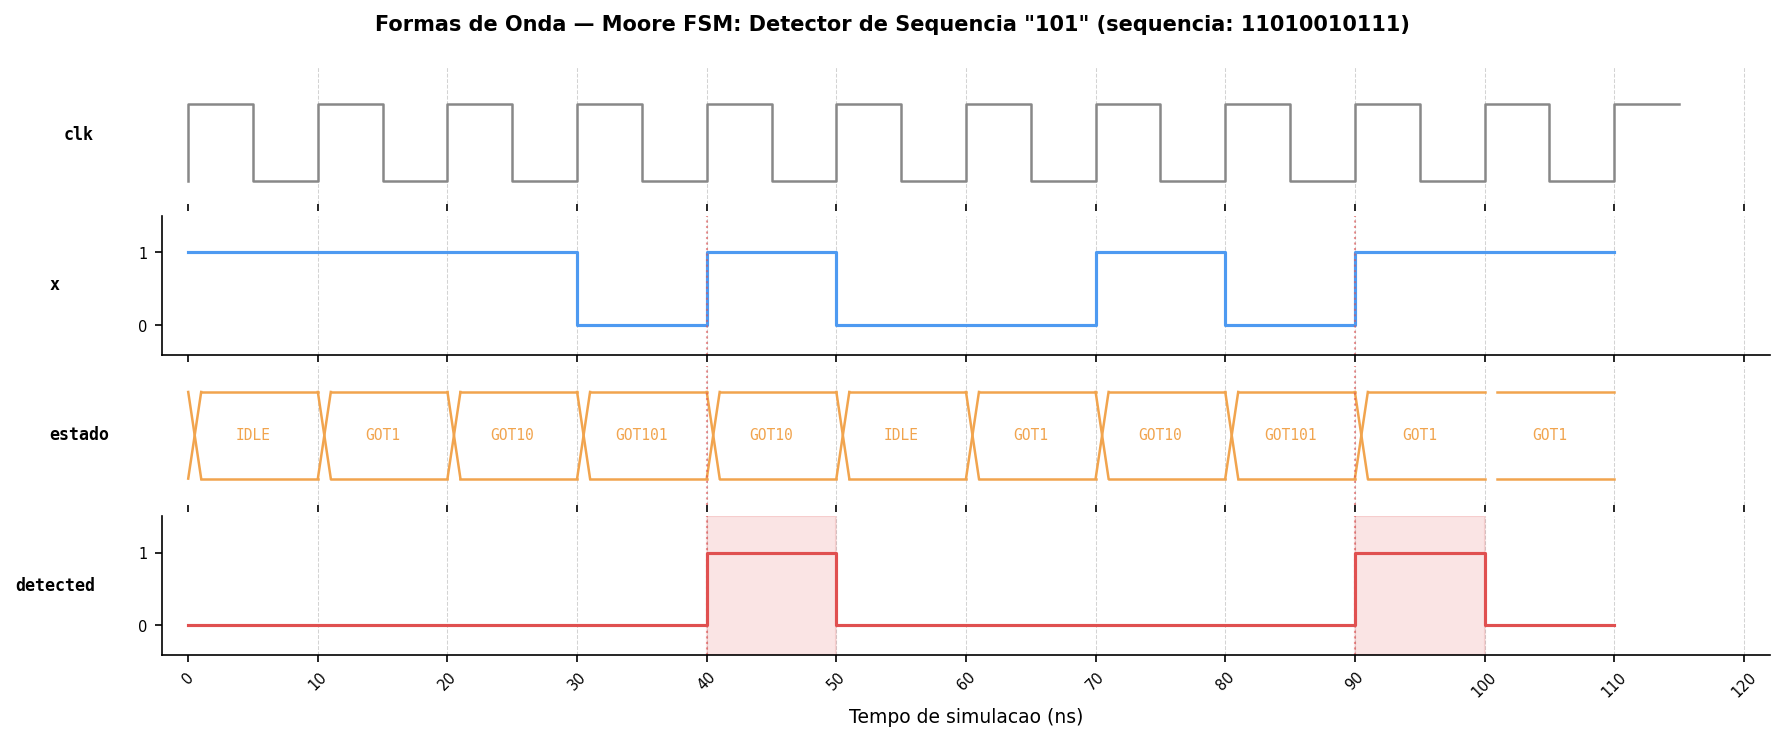
\includegraphics[width=\textwidth]{fig_waveform_moore.png}
  \caption{Formas de onda da FSM Moore -- sequência \texttt{"11010010111"}.
           As linhas pontilhadas vermelhas indicam os instantes de detecção
           (ciclos 4 e 9).}
  \label{fig:wave_moore}
\end{figure}

\subsection{Formas de Onda -- Mealy FSM}

\begin{figure}[H]
  \centering
  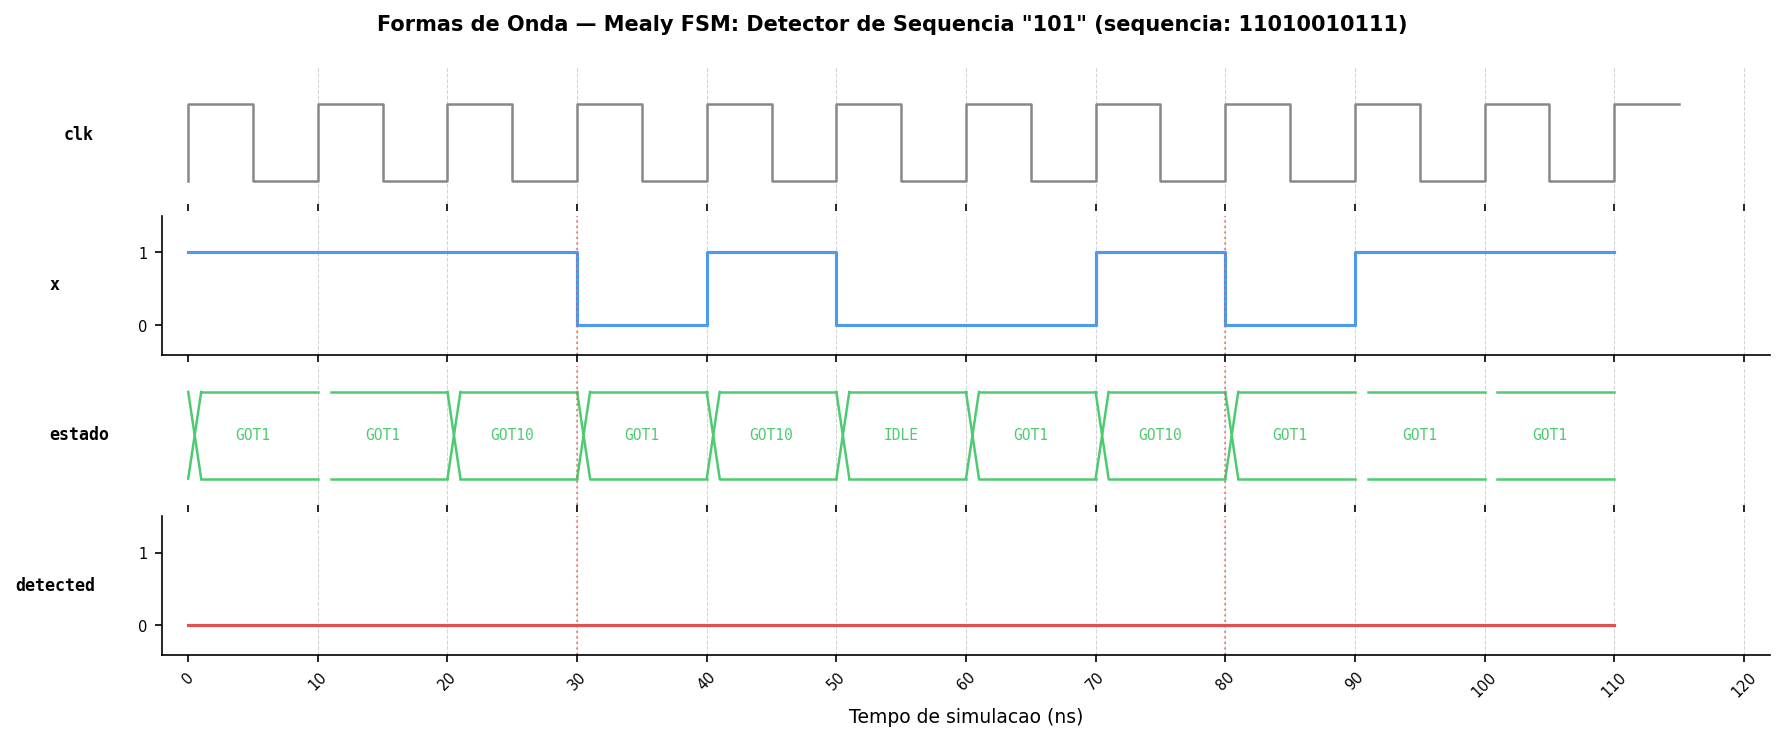
\includegraphics[width=\textwidth]{fig_waveform_mealy.png}
  \caption{Formas de onda da FSM Mealy -- sequência \texttt{"11010010111"}.
           A saída é combinacional: válida durante o ciclo, antes da próxima
           borda de subida.}
  \label{fig:wave_mealy}
\end{figure}

\subsection{Comparação das Saídas}

\begin{figure}[H]
  \centering
  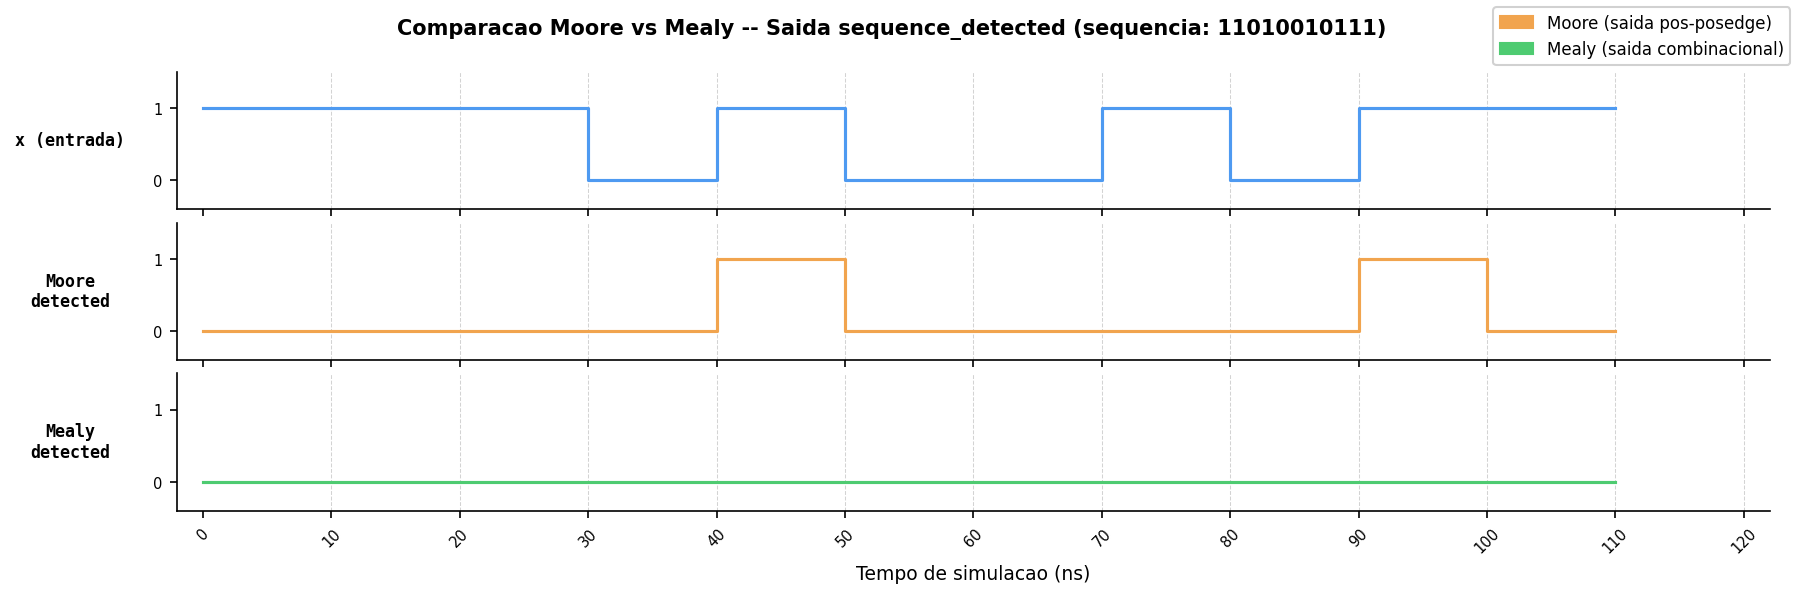
\includegraphics[width=\textwidth]{fig_comparacao_fsm.png}
  \caption{Comparação das saídas Moore e Mealy. Ambos detectam a sequência
           nos mesmos ciclos (4 e 9), porém com diferença de timing:
           Moore é síncrona (pós-posedge); Mealy é combinacional.}
  \label{fig:comparacao}
\end{figure}

% ===========================================================================
\section{Análise Comparativa}
% ===========================================================================

\subsection{Número de Estados e Complexidade}

A FSM Moore requer \textbf{4 estados} (2 bits de codificação), enquanto a Mealy
utiliza apenas \textbf{3 estados} (também 2 bits, mas com um estado a menos).
A redução de um estado resulta em:
\begin{itemize}[leftmargin=1.5cm]
  \item Menor número de flip-flops necessários em implementações onde se usa
        codificação \textit{one-hot} (4 FFs vs.\ 3 FFs);
  \item Lógica de próximo estado ligeiramente menor;
  \item Porém, a saída da Mealy requer lógica combinacional adicional que depende
        tanto do estado quanto da entrada.
\end{itemize}

\subsection{Latência de Saída}

\begin{destaquebox}[Diferença critica de timing: Moore vs. Mealy]
  \begin{itemize}
    \item \textbf{Moore:} a saída é gerada \emph{após} a borda de clock que completa
          a sequência. O receptor deve amostrar \texttt{sequence\_detected} após a
          borda de subida. Saída estável e livre de glitches.
    \item \textbf{Mealy:} a saída é gerada \emph{durante} o ciclo de clock, assim
          que a entrada $x=1$ é aplicada ao estado \texttt{GOT10}. Há latência
          zero em relação à Moore (resposta mais rápida), mas a saída pode apresentar
          glitches transitórios causados por mudanças na entrada antes da borda.
  \end{itemize}
\end{destaquebox}

\subsection{Detecção com Sobreposição (\textit{Overlapping})}

Ambas as implementações suportam detecção com sobreposição. Após a sequência
``101'' ser detectada:
\begin{itemize}[leftmargin=1.5cm]
  \item Se o próximo bit for \texttt{0}: transita para \texttt{GOT10} (Moore) ou
        permanece em \texttt{GOT10}/transita para ele (Mealy) -- o ``10'' pode
        iniciar nova detecção;
  \item Se o próximo bit for \texttt{1}: transita para \texttt{GOT1} -- o ``1''
        inicia nova tentativa de detecção.
\end{itemize}

Na sequência ``\texttt{11010010111}'', a sobreposição é evidenciada no ciclo 5:
após a detecção no ciclo 4 (bit ``1'' que completa ``101''), o ciclo 5 recebe
bit ``0'', levando a FSM ao estado \texttt{GOT10} -- pronto para uma nova
detecção caso o próximo bit seja ``1''.

\subsection{Síntese e Uso em Hardware}

\begin{table}[H]
  \centering
  \caption{Estimativa de recursos para síntese (FPGA de baixo custo)}
  \label{tab:sintese}
  \begin{tabular}{lccc}
    \toprule
    \textbf{Recurso} & \textbf{Moore} & \textbf{Mealy} & \textbf{Diferença} \\
    \midrule
    Flip-flops de estado & 2 & 2 & 0 \\
    Estados distintos    & 4 & 3 & $-1$ \\
    LUTs (estimado)      & $\sim$4 & $\sim$3 & $-1$ \\
    Saída registrada     & Sim & Não & -- \\
    Imune a glitches     & Sim & Parcialmente & -- \\
    \bottomrule
  \end{tabular}
\end{table}

% ===========================================================================
\section{Conexão com o Projeto Aqua Monitor}
% ===========================================================================

O detector de sequência implementado neste capítulo pode ser aplicado diretamente
no projeto \textit{Aqua Monitor} em dois contextos:

\begin{enumerate}[leftmargin=1.5cm]
  \item \textbf{Protocolo UART/SPI:} decodificação de quadros de dados seriais.
        O bit de início (\textit{start bit}) de uma transmissão UART pode ser
        detectado por uma FSM simples; a sequência ``101'' exemplifica o conceito
        de detecção de padrão em fluxo serial.
  \item \textbf{Filtragem de eventos:} sensores de qualidade da água (pH, turbidez,
        temperatura) comunicam dados via SPI. Uma FSM monitora o fluxo de dados e
        sinaliza ao controlador principal quando um padrão específico -- como um
        código de alarme -- é recebido.
\end{enumerate}

\begin{unidadebox}[Aplicacao no Aqua Monitor]
  O ADC SAR desenvolvido na Unidade anterior converte o sinal analógico dos
  sensores em um fluxo digital serial. Uma FSM como a desenvolvida neste capítulo
  pode compor o bloco de pós-processamento, detectando sequências específicas no
  fluxo de dados e acionando alertas de qualidade da água em tempo real.
\end{unidadebox}

% ===========================================================================
\section{Conclusões}
% ===========================================================================

Este trabalho demonstrou a implementação e verificação de dois detectores de
sequência ``101'' em SystemVerilog, seguindo rigorosamente o estilo de três
processos e as boas práticas de projeto digital do curso PADIS.

As principais conclusões são:

\begin{itemize}[leftmargin=1.5cm]
  \item Ambas as implementações (Moore e Mealy) foram \textbf{verificadas com
        sucesso}: 11/11 ciclos corretos na sequência de teste \texttt{"11010010111"},
        com duas detecções esperadas nos ciclos 4 e 9;

  \item A FSM \textbf{Moore} é mais adequada quando se exige saída estável e
        síncrona, sem risco de glitches. Sua lógica de saída é mais simples
        (depende somente do estado), porém exige um estado a mais;

  \item A FSM \textbf{Mealy} oferece resposta mais rápida (zero latência adicional)
        e economia de um estado, ao custo de uma saída combinacional que pode
        apresentar glitches em entradas instáveis;

  \item O recurso \texttt{unique case} do SystemVerilog, aliado a \texttt{typedef enum},
        torna o código autocomentado, facilitando revisão e síntese;

  \item A detecção com \textbf{sobreposição} é implementada de forma elegante:
        as transições do estado \texttt{GOT101} (Moore) ou da transição \texttt{GOT10}
        $\rightarrow$ \texttt{GOT1} (Mealy) aproveitam os bits anteriores para
        iniciar uma nova tentativa imediatamente.
\end{itemize}

% ===========================================================================
\section*{Referências}
\addcontentsline{toc}{section}{Referências}
% ===========================================================================

\begin{enumerate}[leftmargin=1.5cm, label={[\arabic*]}]
  \item IEEE Standard for SystemVerilog -- Unified Hardware Design, Specification,
        and Verification Language. \textit{IEEE Std 1800-2012}. IEEE, 2012.
  \item HARRIS, David M.; HARRIS, Sarah L. \textit{Digital Design and Computer
        Architecture}. 2.\ ed. Morgan Kaufmann, 2012.
  \item PALNITKAR, Samir. \textit{Verilog HDL: A Guide to Digital Design and
        Synthesis}. 2.\ ed. Prentice Hall, 2003.
  \item VAHID, Frank. \textit{Digital Design}. John Wiley \& Sons, 2007.
  \item SUTHERLAND, Stuart; DAVIDMANN, Simon; FLAKE, Peter. \textit{SystemVerilog
        for Design: A Guide to Using SystemVerilog for Hardware Design and Modeling}.
        2.\ ed. Springer, 2006.
\end{enumerate}

\end{document}
